\pdfoutput=1

%\documentclass[preprint,10pt]{elsarticle}
%\documentclass[preprint,10pt]{article}
\documentclass[review]{siamart0216}
%\documentclass{siamart0216}

%\usepackage{fullpage}
%\usepackage[colorlinks=true]{hyperref}

\usepackage{amsmath,amssymb,amsfonts}
%\usepackage{amsthm}
%\theoremstyle{definition}
%\newtheorem{definition}{Definition}
%\theoremstyle{lemma}
%\newtheorem{lemma}{Lemma}
%\theoremstyle{corollary}
%\newtheorem{corollary}{Corollary}
%\theoremstyle{theorem}
%\newtheorem{theorem}{Theorem}
\newtheorem*{remark}{Remark}
\theoremstyle{assumption}
\newtheorem{assumption}{Assumption}

\usepackage[titletoc,toc,title]{appendix}

\usepackage{array} 
\usepackage{listings}
\usepackage{mathtools}
\usepackage{pdfpages}
\usepackage[textsize=footnotesize,color=green]{todonotes}
\usepackage{bm}
\usepackage{bbm}

\usepackage{tikz}
\usepackage[normalem]{ulem}
\usepackage{hhline}

\usepackage{graphicx}
\usepackage{subfig}
\usepackage{color}

%% ====================================== graphics

\usepackage{pgfplots}
\usepackage{pgfplotstable}
\definecolor{markercolor}{RGB}{124.9, 255, 160.65}
\pgfplotsset{
compat=1.3,
width=10cm,
tick label style={font=\small},
label style={font=\small},
legend style={font=\small}
}

\usetikzlibrary{calc}
\usetikzlibrary{intersections} 

%%% START MACRO FOR ANNOTATION OF TRIANGLE WITH SLOPE %%%.
\newcommand{\logLogSlopeTriangle}[5]
{
    % #1. Relative offset in x direction.
    % #2. Width in x direction, so xA-xB.
    % #3. Relative offset in y direction.
    % #4. Slope d(y)/d(log10(x)).
    % #5. Plot options.

    \pgfplotsextra
    {
        \pgfkeysgetvalue{/pgfplots/xmin}{\xmin}
        \pgfkeysgetvalue{/pgfplots/xmax}{\xmax}
        \pgfkeysgetvalue{/pgfplots/ymin}{\ymin}
        \pgfkeysgetvalue{/pgfplots/ymax}{\ymax}

        % Calculate auxilliary quantities, in relative sense.
        \pgfmathsetmacro{\xArel}{#1}
        \pgfmathsetmacro{\yArel}{#3}
        \pgfmathsetmacro{\xBrel}{#1-#2}
        \pgfmathsetmacro{\yBrel}{\yArel}
        \pgfmathsetmacro{\xCrel}{\xArel}

        \pgfmathsetmacro{\lnxB}{\xmin*(1-(#1-#2))+\xmax*(#1-#2)} % in [xmin,xmax].
        \pgfmathsetmacro{\lnxA}{\xmin*(1-#1)+\xmax*#1} % in [xmin,xmax].
        \pgfmathsetmacro{\lnyA}{\ymin*(1-#3)+\ymax*#3} % in [ymin,ymax].
        \pgfmathsetmacro{\lnyC}{\lnyA+#4*(\lnxA-\lnxB)}
        \pgfmathsetmacro{\yCrel}{\lnyC-\ymin)/(\ymax-\ymin)} % THE IMPROVED EXPRESSION WITHOUT 'DIMENSION TOO LARGE' ERROR.

        % Define coordinates for \draw. MIND THE 'rel axis cs' as opposed to the 'axis cs'.
        \coordinate (A) at (rel axis cs:\xArel,\yArel);
        \coordinate (B) at (rel axis cs:\xBrel,\yBrel);
        \coordinate (C) at (rel axis cs:\xCrel,\yCrel);

        % Draw slope triangle.
        \draw[#5]   (A)-- node[pos=0.5,anchor=north] {}
                    (B)-- 
                    (C)-- node[pos=0.5,anchor=west] {\textcolor{black}{#4}}
                    cycle;
    }
}
%%% END MACRO FOR ANNOTATION OF TRIANGLE WITH SLOPE %%%.

\newcommand{\logLogSlopeTriangleNeg}[5]
{
    % #1. Relative offset in x direction.
    % #2. Width in x direction, so xA-xB.
    % #3. Relative offset in y direction.
    % #4. Slope d(y)/d(log10(x)).
    % #5. Plot options.

    \pgfplotsextra
    {
        \pgfkeysgetvalue{/pgfplots/xmin}{\xmin}
        \pgfkeysgetvalue{/pgfplots/xmax}{\xmax}
        \pgfkeysgetvalue{/pgfplots/ymin}{\ymin}
        \pgfkeysgetvalue{/pgfplots/ymax}{\ymax}

        % Calculate auxilliary quantities, in relative sense.
        \pgfmathsetmacro{\xArel}{#1}
        \pgfmathsetmacro{\yArel}{#3}
        \pgfmathsetmacro{\xBrel}{#1-#2}
        \pgfmathsetmacro{\yBrel}{\yArel}
        \pgfmathsetmacro{\xCrel}{\xArel}

        \pgfmathsetmacro{\lnxB}{\xmin*(1-(#1-#2))+\xmax*(#1-#2)} % in [xmin,xmax].
        \pgfmathsetmacro{\lnxA}{\xmin*(1-#1)+\xmax*#1} % in [xmin,xmax].
        \pgfmathsetmacro{\lnyA}{\ymin*(1-#3)+\ymax*#3} % in [ymin,ymax].
        \pgfmathsetmacro{\lnyC}{\lnyA+#4*(\lnxA-\lnxB)}
        \pgfmathsetmacro{\yCrel}{\lnyC-\ymin)/(\ymax-\ymin)} % THE IMPROVED EXPRESSION WITHOUT 'DIMENSION TOO LARGE' ERROR.

        % Define coordinates for \draw. MIND THE 'rel axis cs' as opposed to the 'axis cs'.
        \coordinate (A) at (rel axis cs:\xArel,\yArel);
        \coordinate (B) at (rel axis cs:\xBrel,\yBrel);
        \coordinate (C) at (rel axis cs:\xCrel,\yCrel);

        % Draw slope triangle.
        \draw[#5]   (A)-- node[pos=.5,anchor=south] {}
                    (B)-- 
                    (C)-- node[pos=0.5,anchor=west] {\textcolor{black}{#4}}
                    cycle;
    }
}
%%% END MACRO FOR ANNOTATION OF TRIANGLE WITH SLOPE %%%.

%%% START MACRO FOR ANNOTATION OF TRIANGLE WITH SLOPE %%%.
\newcommand{\logLogSlopeTriangleFlipNeg}[5]
{
    % #1. Relative offset in x direction.
    % #2. Width in x direction, so xA-xB.
    % #3. Relative offset in y direction.
    % #4. Slope d(y)/d(log10(x)).
    % #5. Plot options.

    \pgfplotsextra
    {
        \pgfkeysgetvalue{/pgfplots/xmin}{\xmin}
        \pgfkeysgetvalue{/pgfplots/xmax}{\xmax}
        \pgfkeysgetvalue{/pgfplots/ymin}{\ymin}
        \pgfkeysgetvalue{/pgfplots/ymax}{\ymax}

        % Calculate auxilliary quantities, in relative sense.
        %\pgfmathsetmacro{\xArel}{#1}
        %\pgfmathsetmacro{\yArel}{#3}
        \pgfmathsetmacro{\xBrel}{#1-#2}
        \pgfmathsetmacro{\yBrel}{#3}
        \pgfmathsetmacro{\xCrel}{#1}

        \pgfmathsetmacro{\lnxB}{\xmin*(1-(#1-#2))+\xmax*(#1-#2)} % in [xmin,xmax].
        \pgfmathsetmacro{\lnxA}{\xmin*(1-#1)+\xmax*#1} % in [xmin,xmax].
        \pgfmathsetmacro{\lnyA}{\ymin*(1-#3)+\ymax*#3} % in [ymin,ymax].
        \pgfmathsetmacro{\lnyC}{\lnyA+#4*(\lnxA-\lnxB)}
        \pgfmathsetmacro{\yCrel}{\lnyC-\ymin)/(\ymax-\ymin)} % THE IMPROVED EXPRESSION WITHOUT 'DIMENSION TOO LARGE' ERROR.

	\pgfmathsetmacro{\xArel}{\xBrel}
        \pgfmathsetmacro{\yArel}{\yCrel}

        % Define coordinates for \draw. MIND THE 'rel axis cs' as opposed to the 'axis cs'.
        \coordinate (A) at (rel axis cs:\xArel,\yArel);
        \coordinate (B) at (rel axis cs:\xBrel,\yBrel);
        \coordinate (C) at (rel axis cs:\xCrel,\yCrel);

        % Draw slope triangle.
        \draw[#5]   (A)-- node[pos=0.5,anchor=east] {\textcolor{black}{#4}}
                    (B)-- 
                    (C)-- node[pos=0.5,anchor=north] {1}
                    cycle;
    }
}
%%% END MACRO FOR ANNOTATION OF TRIANGLE WITH SLOPE %%%.


%%% START MACRO FOR ANNOTATION OF TRIANGLE WITH SLOPE %%%.
\newcommand{\logLogSlopeTriangleFlip}[5]
{
    % #1. Relative offset in x direction.
    % #2. Width in x direction, so xA-xB.
    % #3. Relative offset in y direction.
    % #4. Slope d(y)/d(log10(x)).
    % #5. Plot options.

    \pgfplotsextra
    {
        \pgfkeysgetvalue{/pgfplots/xmin}{\xmin}
        \pgfkeysgetvalue{/pgfplots/xmax}{\xmax}
        \pgfkeysgetvalue{/pgfplots/ymin}{\ymin}
        \pgfkeysgetvalue{/pgfplots/ymax}{\ymax}

        % Calculate auxilliary quantities, in relative sense.
        %\pgfmathsetmacro{\xArel}{#1}
        %\pgfmathsetmacro{\yArel}{#3}
        \pgfmathsetmacro{\xBrel}{#1-#2}
        \pgfmathsetmacro{\yBrel}{#3}
        \pgfmathsetmacro{\xCrel}{#1}

        \pgfmathsetmacro{\lnxB}{\xmin*(1-(#1-#2))+\xmax*(#1-#2)} % in [xmin,xmax].
        \pgfmathsetmacro{\lnxA}{\xmin*(1-#1)+\xmax*#1} % in [xmin,xmax].
        \pgfmathsetmacro{\lnyA}{\ymin*(1-#3)+\ymax*#3} % in [ymin,ymax].
        \pgfmathsetmacro{\lnyC}{\lnyA+#4*(\lnxA-\lnxB)}
        \pgfmathsetmacro{\yCrel}{\lnyC-\ymin)/(\ymax-\ymin)} % THE IMPROVED EXPRESSION WITHOUT 'DIMENSION TOO LARGE' ERROR.

	\pgfmathsetmacro{\xArel}{\xBrel}
        \pgfmathsetmacro{\yArel}{\yCrel}

        % Define coordinates for \draw. MIND THE 'rel axis cs' as opposed to the 'axis cs'.
        \coordinate (A) at (rel axis cs:\xArel,\yArel);
        \coordinate (B) at (rel axis cs:\xBrel,\yBrel);
        \coordinate (C) at (rel axis cs:\xCrel,\yCrel);

        % Draw slope triangle.
        \draw[#5]   (A)-- node[pos=0.5,anchor=east] {\textcolor{black}{#4}}
                    (B)-- 
                    (C)-- node[pos=0.5,anchor=south] {}
                    cycle;
    }
}
%%% END MACRO FOR ANNOTATION OF TRIANGLE WITH SLOPE %%%.



\usepackage{stmaryrd}

\renewcommand{\hat}[1]{\widehat{#1}}
\renewcommand{\topfraction}{0.85}
\renewcommand{\textfraction}{0.1}
\renewcommand{\floatpagefraction}{0.75}

\newcommand{\vect}[1]{\ensuremath\boldsymbol{#1}}
\newcommand{\tensor}[1]{\underline{\bm{#1}}}
\newcommand{\del}{\triangle}
\newcommand{\curl}{\grad \times}
\renewcommand{\div}{\grad \cdot}

\newcommand{\bbm}[1]{\mathbbm{#1}}
\newcommand{\bs}[1]{\boldsymbol{#1}}
\newcommand{\equaldef}{\stackrel{\mathrm{def}}{=}}

\newcommand{\td}[2]{\frac{{\rm d}#1}{{\rm d}{\rm #2}}}
\newcommand{\pd}[2]{\frac{\partial#1}{\partial#2}}
\newcommand{\nor}[1]{\left\| #1 \right\|}
\newcommand{\LRp}[1]{\left( #1 \right)}
\newcommand{\LRs}[1]{\left[ #1 \right]}
\newcommand{\LRa}[1]{\left\langle #1 \right\rangle}
\newcommand{\LRb}[1]{\left| #1 \right|}
\newcommand{\LRc}[1]{\left\{ #1 \right\}}
\newcommand{\LRceil}[1]{\left\lceil #1 \right\rceil}
\newcommand{\LRl}[1]{\left. #1 \right|}
\newcommand{\pdd}[2]{\frac{\partial^2#1}{\partial#2^2}}
\newcommand{\pdn}[3]{\frac{\partial^{#3}#1}{\partial#2^{#3}}}
\newcommand{\mb}[1]{\mathbf{#1}}
\newcommand{\mbb}[1]{\mathbb{#1}}
\newcommand{\mc}[1]{\mathcal{#1}}
\newcommand{\snor}[1]{\left| #1 \right|}


%\newcommand{\cond}[1]{\kappa\LRp{#1}}
\newcommand{\cond}[2]{\nor{#1}_{#2}\nor{{#1}^{-1}}_{#2}}


\newcommand{\Grad} {\ensuremath{\nabla}}
\newcommand{\Div} {\ensuremath{\nabla\cdot}}
\newcommand{\jump}[1] {\ensuremath{\llbracket#1\rrbracket}}
\newcommand{\avg}[1] {\ensuremath{\LRc{\!\{#1\}\!}}}

\newcommand{\Oh}{{\Omega_h}}
\renewcommand{\L}{L^2\LRp{\Omega}}
\newcommand{\LK}{L^2\LRp{D^k}}
\newcommand{\LdK}{L^2\LRp{\partial D^k}}
\newcommand{\Dhat}{\widehat{D}}
\newcommand{\Lhat}{L^2\LRp{\Dhat}}

\newcommand{\eval}[2][\right]{\relax
  \ifx#1\right\relax \left.\fi#2#1\rvert}

\def\etal{{\it et al.~}}


\newcommand{\note}[1]{{\color{blue}{#1}}}
%\newcommand{\noteOne}[1]{{\color{blue}{#1}}}
%\newcommand{\noteTwo}[1]{{\color{red}{#1}}}
%\newcommand{\note}[1]{#1}
%\newcommand{\noteOne}[1]{#1}
%\newcommand{\noteTwo}[1]{#1}


\newcommand{\LinfDk}{L^{\infty}\LRp{D^k}}

\newcommand{\diag}[1]{{\rm diag}\LRp{#1}}

\newcommand{\Ksub}{K_{\rm sub}}

\newcolumntype{C}[1]{>{\centering\let\newline\\\arraybackslash\hspace{0pt}}m{#1}}

%% d in integrand
\newcommand*\diff[1]{\mathop{}\!{\mathrm{d}#1}}

\makeatletter
\renewcommand\d[1]{\mspace{6mu}\mathrm{d}#1\@ifnextchar\d{\mspace{-3mu}}{}}
\makeatother

\date{}
\author{Jesse Chan}%, David C.\ Del Rey Fernandez}
\title{Skew-symmetric entropy stable discontinuous Galerkin formulations with applications to hybrid and non-conforming meshes}

\graphicspath{{./figs/}}

\begin{document}

\maketitle

%\begin{frontmatter}
%\title{Entropy stable skew-symmetric discontinuous Galerkin formulations with applications to hybrid and non-conforming meshes. }
%
%\author[rice]{Jesse Chan\corref{cor1}}
%\ead{Jesse.Chan@caam.rice.edu}
%\address[rice]{Department of Computational and Applied Mathematics, Rice University, 6100 Main St, Houston, TX, 77005}
%
%\begin{abstract}
%Entropy stable high order methods for nonlinear conservation laws satisfy an inherent discrete entropy inequality.  
%\end{abstract}
%\end{frontmatter}

%\tableofcontents

\section{Introduction}

High order methods for the simulation of time-dependent compressible flow have the potential to achieve higher levels of accuracy at lower costs compared to current low order schemes \cite{wang2013high}.  In addition to superior accuracy and efficiency on modern computing architectures, the low numerical dispersion and dissipation of high order methods \cite{ainsworth2004dispersive} enables the accurate propagation of waves over long distances and time scales.  The same properties also make high order methods attractive for the resolution of unsteady phenomena such as vorticular and turbulent flows, which are sensitive to numerical dissipation \cite{visbal1999high, wang2013high}.  However, while high order methods are often provably stable for wave problems, high order schemes for nonlinear conservation laws have consistently been hampered by problems of instability.  

When applied to nonlinear conservation laws, high order methods can experience artificial growth and blow-up near under-resolved features such as shocks, turbulence, or boundary layers.  In practice, the application of high order methods to practical problems requires shock capturing and stabilization techniques (such as artificial viscosity) or solution regularization (such as filtering or limiting) to prevent solution blow-up.  The resulting schemes for nonlinear conservation laws walk a fine line between stability, robustness, and accuracy.  Aggressive stabilization or regularization can result in the loss of high order accuracy, while too little can result in instability \cite{wang2013high}.  Moreover, it can be difficult to determine robust expressions for stabilization paramaters, as parameters which work for one simulation can fail when applied to a different physical regime or discretization setting.  

These issues have motivated the introduction of high order \textit{entropy stable} discretizations, which satisfy a semi-discrete entropy inequality while maintaining high order accuracy in smooth regions.  Proofs of continuous entropy inequalities rely on the chain rule.  In contrast, these discrete entropy inequalities account for the loss of the chain rule due to effects such as quadrature errors, which are incurred when applying polynomially exact quadrature rules to nonlinear and rational integrands within the DG formulation.  These schemes were first introduced as high order collocation methods on tensor product elements in \cite{fisher2013high, carpenter2014entropy, gassner2016split, gassner2017br1}, and were extended to simplicial elements in \cite{crean2017high, chen2017entropy, crean2018entropy, chan2017discretely}.  These methods have also been extended to staggered grid methods \cite{parsani2016entropy} and non-conforming meshes \cite{friedrich2017entropy}.  Entropy stable boundary conditions have also been determined for the compressible Euler and Navier-Stokes equations \cite{parsani2015entropy, svard2018entropy}.  

\section{Entropy stability for systems of nonlinear conservation laws}

We begin by reviewing the dissipation of entropy for a $d$-dimensional system of nonlinear conservation laws on a domain $\Omega$
\begin{equation}
\pd{\bm{u}}{t}  + \sum_{j=1}^d\pd{\bm{f}_j(\bm{u})}{x_j} = 0, \qquad \bm{u}\in \mathbb{R}^n, \qquad \bm{f}:\mathbb{R}^n\rightarrow\mathbb{R}^n,
\label{eq:nonlineqs}
\end{equation}
where $\bm{u}$ are the conservative variables and $\bm{f}(\bm{u})$ is a vector-valued nonlinear flux function.  We are interested in nonlinear conservation laws for which a convex entropy function $U(\bm{u})$ exists.  For such systems, the  \emph{entropy variables} are an invertible mapping $\bm{v}(\bm{u}):\mathbb{R}^n\rightarrow \mathbb{R}^n$ defined as the derivative of the entropy function with respect to the conservative variables 
\begin{align}
\bm{v}(\bm{u}) = \pd{U}{\bm{u}}.%, \qquad  \text{ invertible}.%\bm{u}\LRp{\bm{v}(\bm{u})} = \bm{u}.
\label{eq:entropyvarsmap}
\end{align}
Several widely used equations in fluid modeling (Burgers, shallow water, compressible Euler and Navier-Stokes equations) yield convex entropy functions $U(\bm{u})$ \cite{hughes1986new, chen2017entropy}.  Let $\partial \Omega$ be the boundary of $\Omega$ with outward unit normal $\bm{n}$.  By multiplying the equation (\ref{eq:nonlineqs}) with $\bm{v}(\bm{u})^T$, the solutions $\bm{u}$ of (\ref{eq:nonlineqs}) can be shown to satisfy an entropy inequality
\begin{equation}
\int_{\Omega}\pd{U(\bm{u})}{t}\diff{x} + \int_{\partial \Omega} \sum_{j=1}^d \LRp{\bm{v}(\bm{u})^T\bm{f}_j(\bm{u}) - \psi_j\LRp{\bm{v}(\bm{u})}}n_j \diff{x} \leq 0, 
\label{eq:entropyineq}
\end{equation}
where $\bm{n} = \LRp{n_1,\ldots,n_d}$ denotes the outward unit normal, and $\psi_j(\bm{u})$ is some function referred to as the entropy potential.  

The proof of (\ref{eq:entropyineq}) requires the use of the chain rule \cite{mock1980systems, harten1983symmetric, dafermos2005compensated}.  The instability-in-practice of high order schemes for (\ref{eq:nonlineqs}) can be attributed in part to the fact that the discrete form of the equations do not satisfy the chain rule, and thus do not satisfy (\ref{eq:entropyineq}).  As a result, discretizations of (\ref{eq:nonlineqs}) do not typically possess an underlying statement of stability.  For low order schemes, this can be offset in practice by the inherent numerical dissipation.  However, because high order discretizations possess low numerical dissipation, the lack of an underlying discrete stability has been conflated with the idea that high order methods are inherently less stable than low order methods.

\section{Approximation spaces}

We define an approximation space using degree $N$ polynomials on the reference element.  In this work, we consider either simplicial reference elements (triangles and tetrahedra) or tensor product reference elements (quadrilaterals and hexahedra).  The natural polynomial approximation space differs depending on the element type \cite{chan2015gpu}.  

On a $d$-dimensional reference simplex, the natural polynomial space are total degree $N$ polynomials 
\[
P^N\LRp{\widehat{D}} = \LRc{\hat{x}_1^{i_1}\ldots\hat{x}_d^{i_d}, \quad \hat{\bm{x}} \in \widehat{D}, \quad 0\leq \sum_{k=1}^d i_k \leq N}.
\]
In contrast, the natural polynomial space on a $d$-dimensional tensor product element is 
\[
Q^N\LRp{\widehat{D}} = \LRc{\hat{x}_1^{i_1}\ldots\hat{x}_d^{i_d}, \quad \hat{\bm{x}} \in \widehat{D}, \quad 0\leq i_k \leq N, \quad k = 1,\ldots, d}.
\]
We take $V^N$ to denote the natural approximation space on a given element.  Furthermore, we denote the dimension of $V^N$  as $N_p = {\rm dim}\LRp{V^N\LRp{\widehat{D}}}$.  

We also define trace spaces for each reference element.  Let $\hat{f}$ be a face of the reference element $\hat{D}$.  The trace space $V^N \LRp{\hat{f}}$ is defined as the restrictions of functions in $V^N\LRp{\hat{D}}$ to $\hat{f}$
\[
V^N \LRp{\hat{f}} = \LRc{ \left.u\right|_{\hat{f}}, \quad u \in V^N\LRp{\hat{D}}}, \qquad \hat{f}\in \partial\hat{D}.
\]
For example, the trace space for degree $N$ polynomials on a quadrilateral face $\hat{f}$ of the bi-unit hexahedral element $[-1,1]^3$ is $Q^N\LRp{\hat{f}}$, while the trace space for degree $N$ polynomials on a triangular face $f$ of the tetrahedron is $P^N\LRp{\hat{f}}$.  We denote the dimension of the trace space as ${\rm dim}\LRp{V^N\LRp{{\hat{f}}}} = N^f_p$.  

We similarly define the trace space for the surface $\partial \hat{D}$ of $\hat{D}$
\[
V^N \LRp{\partial \hat{D}} = \LRc{ \left.u\right|_{\partial \hat{D}}, \quad u \in V^N\LRp{\hat{D}}}.
\]



\section{$L^2$ projection and lifting matrices and a decoupled SBP operator}

The schemes in \cite{chan2017discretely} begin on the reference element $\hat{D}$ by approximating the solution in a degree $N$ polynomial basis $\LRc{\phi_j({\bm{x}})}_{i=1}^{N_p}$.  It is assumed that volume and surface quadrature rules $({\bm{x}}_i, w_i)$, $\LRp{{\bm{x}}^f_i,w^f_i}$ are provided for $\hat{D}$ and the surface $\partial \hat{D}$ of $\hat{D}$, respectively.  We make the following assumption on the volume quadrature rule:
\begin{assumption}
The volume quadrature rule integrates exactly all polynomials of degree $(2N-1)$.
\label{ass:quad}
\end{assumption}
In addition to being related to the positive definiteness of the mass matrix, Assumption~\ref{ass:quad} ensures that, for any $u,v \in V^N$, the following integral is exactly approximated using quadrature
\[
\int_{\hat{D}} \pd{u(\hat{\bm{x}})}{\hat{x}_i} v(\hat{\bm{x}})\diff{\hat{\bm{x}}} = \sum_{k=1}^{N_q} w_k \pd{u(\hat{\bm{x}}_k)}{\hat{x}_i} v(\hat{\bm{x}}_k).  
\]
In other words, evaluating the integral of the derivative of $u$ and $v$ using quadrature is exact because the integrand is a polynomial of degree $(2N-1)$.  

\note{TODO: Standardize hat notation for operators/normals: can refer to operators on reference element and do $k$ superscript for physical elements, or do hats on reference element.}

Let $\bm{V}_q,\bm{V}_f$ denote interpolation matrices, and let $\bm{D}^i$ be the differentiation matrix with respect to the $i$th coordinate such that
\begin{gather}
\LRp{\bm{V}_q}_{ij} = \phi_j(\bm{x}_i), \qquad \LRp{\bm{V}_f}_{ij} = \phi_j(\bm{x}^f_i), \qquad \pd{\phi_j(\bm{x})}{x_i} = \sum_{k=1}^{N_p} \LRp{\bm{D}^i_{jk}} \phi_k(\bm{x}).
\end{gather}
The interpolation matrices $\bm{V}_q,\bm{V}_f$ map basis coefficients to evaluations at volume and surface quadrature points respectively, while the differentiation matrix ${\bm{D}}_i$ maps basis coefficients of a function to the basis coefficients of its derivative with respect to $x_k$.  The interpolation matrices are used to assemble the mass matrix $\bm{M}$, the quadrature-based projection matrix $\bm{P}_q$, and lifting matrix $\bm{L}_f$
\begin{gather}
\bm{M} = \bm{V}_q^T\bm{W}\bm{V}_q, \qquad \bm{P}_q = \bm{M}^{-1}\bm{V}_q^T\bm{W}, \qquad \bm{L}_f = \bm{M}^{-1}\bm{V}_f^T\bm{W}_f,
\end{gather}
where $\bm{W}, \bm{W}_f$ are diagonal matrices of volume and surface quadrature weights, respectively.  The matrix $\bm{P}_q$ is a quadrature-based discretization of the $L^2$ projection operator $\Pi_N$ onto degree $N$ polynomials.

Interpolation, differentiation, and $L^2$ projection matrices can be combined to construct finite difference operators.  For example, the matrix $\bm{D}_q = \bm{V}_q\bm{D}^i\bm{P}_q$ maps function values at quadrature points to approximate values of the derivative at quadrature points.  By choosing specific quadrature rules, $\bm{D}_q$ recovers high order summation-by-parts finite difference operators in \cite{gassner2013skew, fernandez2014generalized, ranocha2018generalised} and certain operators in \cite{hicken2016multidimensional}.  However, to address difficulties in designing efficient entropy stable interface terms for nonlinear conservation laws, the PI introduced in \cite{chan2017discretely} a new ``decoupled'' summation by parts matrix which builds interface terms directly into the approximation of the derivative.  

Let $\bm{n}$ denote the outward unit normal $\bm{n}$ on $\hat{D}$, and let $\bm{n}_i$ denote the vector containing values of the $i$th component at all surface quadrature points.  The ``decoupled'' summation by parts operator $\bm{D}^i_N$ is defined as the block matrix involving both volume and surface quadratures
\begin{align}
\bm{D}^i_N  &= \LRs{
\begin{array}{cc}
\bm{D}^i_q - \frac{1}{2}\bm{V}_q \bm{L}_f {\rm diag}({\bm{n}}_i) \bm{V}_f\bm{P}_q &  \frac{1}{2}\bm{V}_q\bm{L}_f{\rm diag}({\bm{n}}_i)\\
-\frac{1}{2}{\rm diag}({\bm{n}}_i)\bm{V}_f\bm{P}_q & \frac{1}{2}{\rm diag}({\bm{n}}_i)
\end{array}}.  
\label{eq:DN}
\end{align}
When combined with projection and lifting matrices, $\bm{D}^i_N$ produces a high order polynomial approximation of $f\pd{g}{x_i}$. 
Let $f, g$ be differentiable functions, and let $\bm{f}_i = f(\bm{x}_i)$, $\bm{g}_i = g(\bm{x}_i)$ denote values of $f,g$ at volume and surface quadrature points.  Then,
\begin{gather}
f\pd{g}{x_i} \approx \LRs{\begin{array}{cc}
\bm{P}_q & \bm{L}_f\end{array}} {\rm diag}\LRp{\bm{f}}\bm{D}^i_N \bm{g}.  
\label{eq:dnapprox}
\end{gather}
The approximation can also be interpreted as solving a variational problem.  Let $n_i$ be the $i$th component of the unit normal on $\hat{D}$.  Then (\ref{eq:dnapprox}) is equivalent to finding $u(\bm{x}) \approx f\pd{g}{x_i}$ such that 
\[
\int_{\hat{D}} u(\bm{x})v(\bm{x})  = \int_{\hat{D}}{g\pd{\Pi_Nf}{x_i}v} + \int_{\partial \hat{D}}{(f-\Pi_Nf)\frac{\LRp{gv + \Pi_N(gv)}}{2}}n_i, \qquad \forall v\in V^N\LRp{\hat{D}}.
\]
If the surface quadrature rule is exact for polynomials of degree $2N$, then the decoupled SBP operator $\bm{D}^i_N$ also satisfies a summation by parts property.  
\begin{gather}
\bm{Q}^i_N = \bm{W}_N \bm{D}^i_N, \qquad \bm{W}_N = \LRp{\begin{array}{cc}\bm{W}&\\ & \bm{W}_f\end{array}},\label{eq:dsbp}\\ \bm{Q}^i_N+\LRp{\bm{Q}^i_N}^T = \LRp{\begin{array}{cc}\bm{0}&\\ & \bm{W}_f {\rm diag}(\bm{n}_i)\end{array}} = \bm{B}_N\nonumber
\end{gather}
By noting that $\bm{W}\bm{V}_q \bm{L}_q = \bm{P}_q^T\bm{V}_f^T\bm{W}_f$, the entries of $\bm{Q}^i_N$ can be re-written as
\begin{align}
\bm{Q}_i &= \bm{W}\bm{V}_q\bm{D}^i\bm{P}_q,\\
\bm{Q}^i_N  &= \LRs{
\begin{array}{cc}
\bm{Q}_i - \frac{1}{2}\LRp{\bm{V}_f \bm{P}_q}^T  \bm{W}_f{\rm diag}({\bm{n}}_i) \bm{V}_f\bm{P}_q &  \frac{1}{2}\LRp{\bm{W}_f{\rm diag}({\bm{n}}_i)\bm{V}_f\bm{P}_q}^T\\
-\frac{1}{2}\bm{W}_f{\rm diag}({\bm{n}}_i)\bm{V}_f\bm{P}_q & \frac{1}{2}\bm{W}_f{\rm diag}({\bm{n}}_i)
\end{array}}.
\label{eq:QN}
\end{align}
from which the SBP property (\ref{eq:dsbp}) is more apparent.  

%\begin{lemma}[Lemma 1 in \cite{chan2017discretely}]
%Let $\bm{D}^i_q = \bm{V}_q\bm{D}^i\bm{P}_q$.  Then, for volume quadratures which are exact for degree $2N-1$ polynomials, $\bm{D}^i_q$ satisfies the SBP property with respect to $\bm{W}$ 
%\[
%\bm{W}\bm{D}^i_q = \LRp{\bm{V}_f\bm{P}_q}^T \bm{W}_f\diag{\hat{\bm{n}}} \bm{V}_f\bm{P}_q - \LRp{\bm{W}\bm{D}^i_q}^T.  
%\]
%\label{lemma:gsbp}
%\end{lemma}


\section{Skew-symmetric entropy conservative formulations}

\subsection{Loss of the SBP property for hybrid and non-conforming meshes}

While the SBP property has been used to derive entropy stable schemes, the SBP property is difficult or impossible to enforce in certain discretization settings, such as hybrid and non-conforming meshes arises.  This difficulty is a result of the choices of surface quadrature which naturally arise for these settings.  

\begin{figure}
\centering
\begingroup
\captionsetup[subfigure]{width=.425\textwidth}
\subfloat[Insufficiently accurate surface quadrature on the triangle element.]{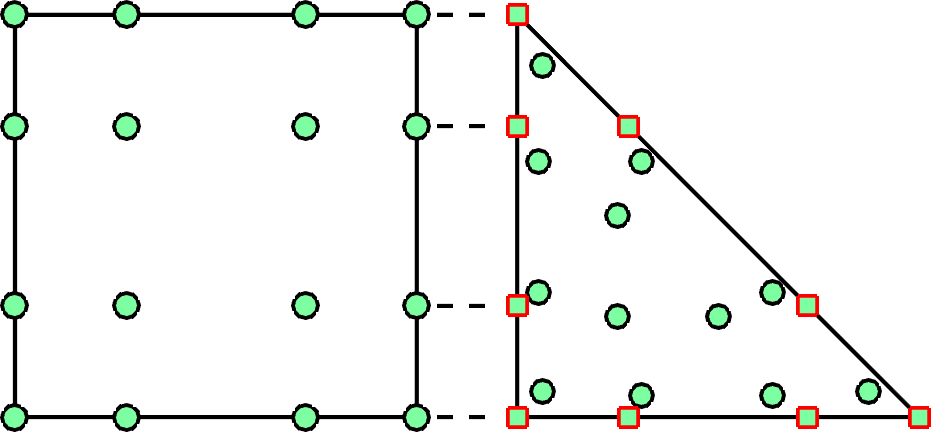
\includegraphics[width=.425\textwidth]{figs/hybrid2D.png}\label{subfig:hybrid1}}
\endgroup
\hspace{2em}
\subfloat[Incompatible surface quadrature on the quadrilateral element.]{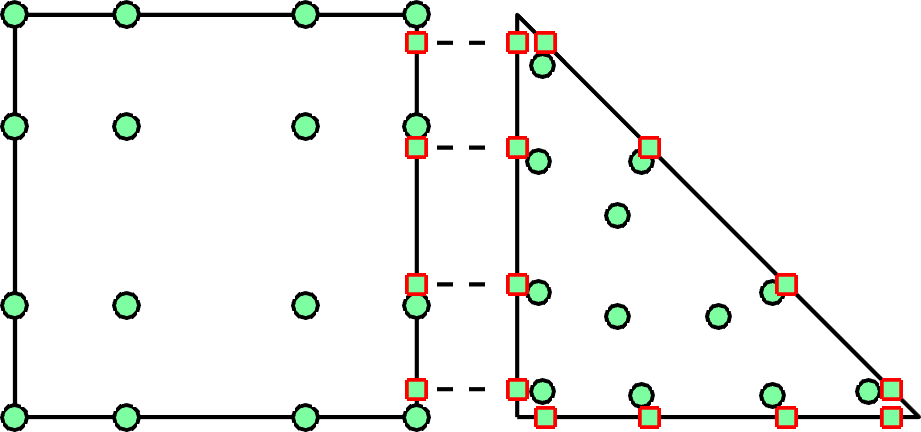
\includegraphics[width=.425\textwidth]{figs/hybrid2D_GQ.png}\label{subfig:hybrid2}}
\caption{Examples of interface couplings which do not result in an SBP property and are not entropy stable.  On the left, the surface quadrature is a $(N+1)$ point GLL rule, and results in a loss of the SBP property on the triangle.  On the right, the surface quadrature is a $(N+1)$ point Gauss-Legendre rule, and results in a loss of the SBP property on the quadrilateral.  }
\label{fig:hybrid}
\end{figure}

\begin{figure}
\centering
\subfloat[Hex-pyramid coupling]{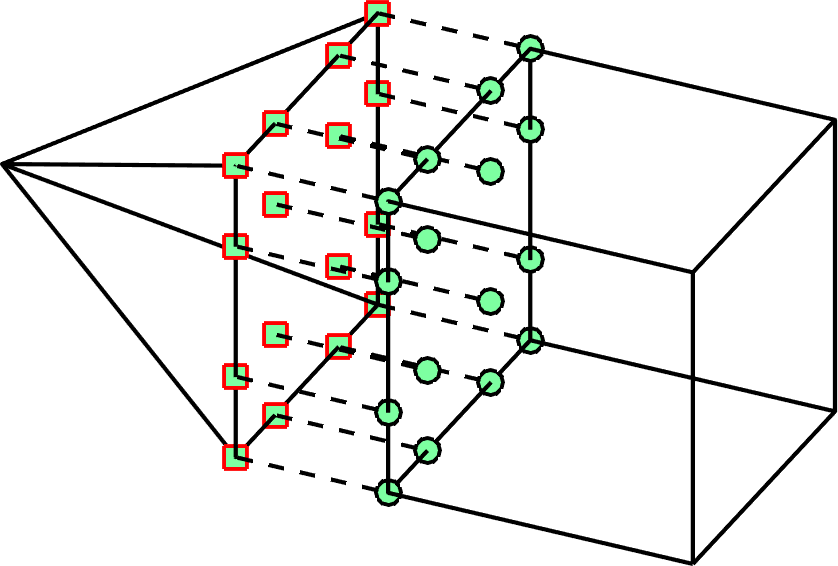
\includegraphics[width=.35\textwidth]{figs/hybrid3D.png}}
\hspace{2em}
\subfloat[Hex-prism coupling]{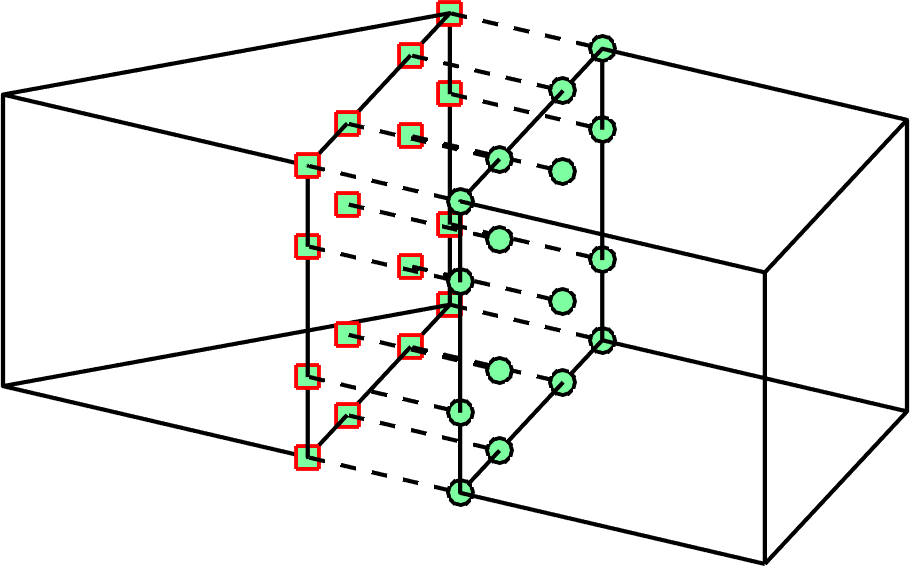
\includegraphics[width=.375\textwidth]{figs/hybrid3D_wedge.png}}
\caption{Illustration of a 3D coupling between a GLL hexahedral element and a pyramid.  The SBP property does not hold on the pyramid due to the use of GLL quadrature on the quadrilateral face. }
\label{fig:hybrid3d}
\end{figure}

\begin{figure}[!h]
\centering
\begingroup
\captionsetup[subfigure]{width=.45\textwidth}
\subfloat[Entropy stable inter-element coupling in \cite{friedrich2017entropy} for a non-conforming interface.]{\raisebox{0em}{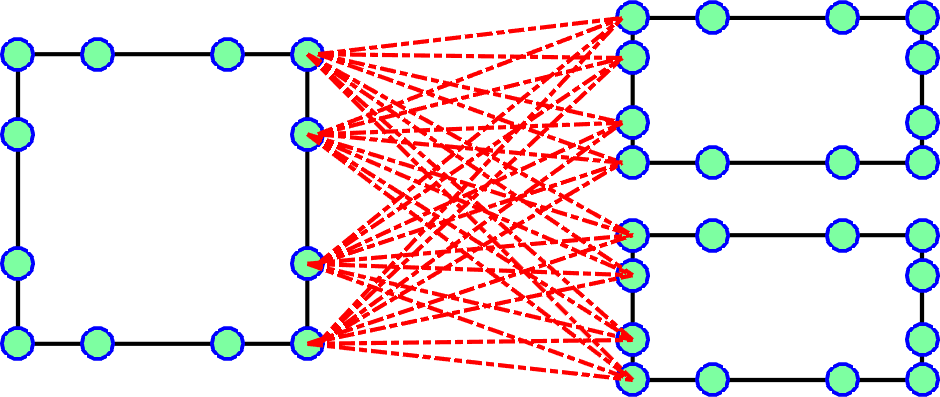
\includegraphics[width=.45\textwidth]{figs/nonconSBP.png}}\label{subfig:noncon2}}
\hspace{2em}
\subfloat[Entropy stable inter-element coupling in this work for a non-conforming interface.  The dotted black lines denote communication between neighboring elements.]{\raisebox{-0em}{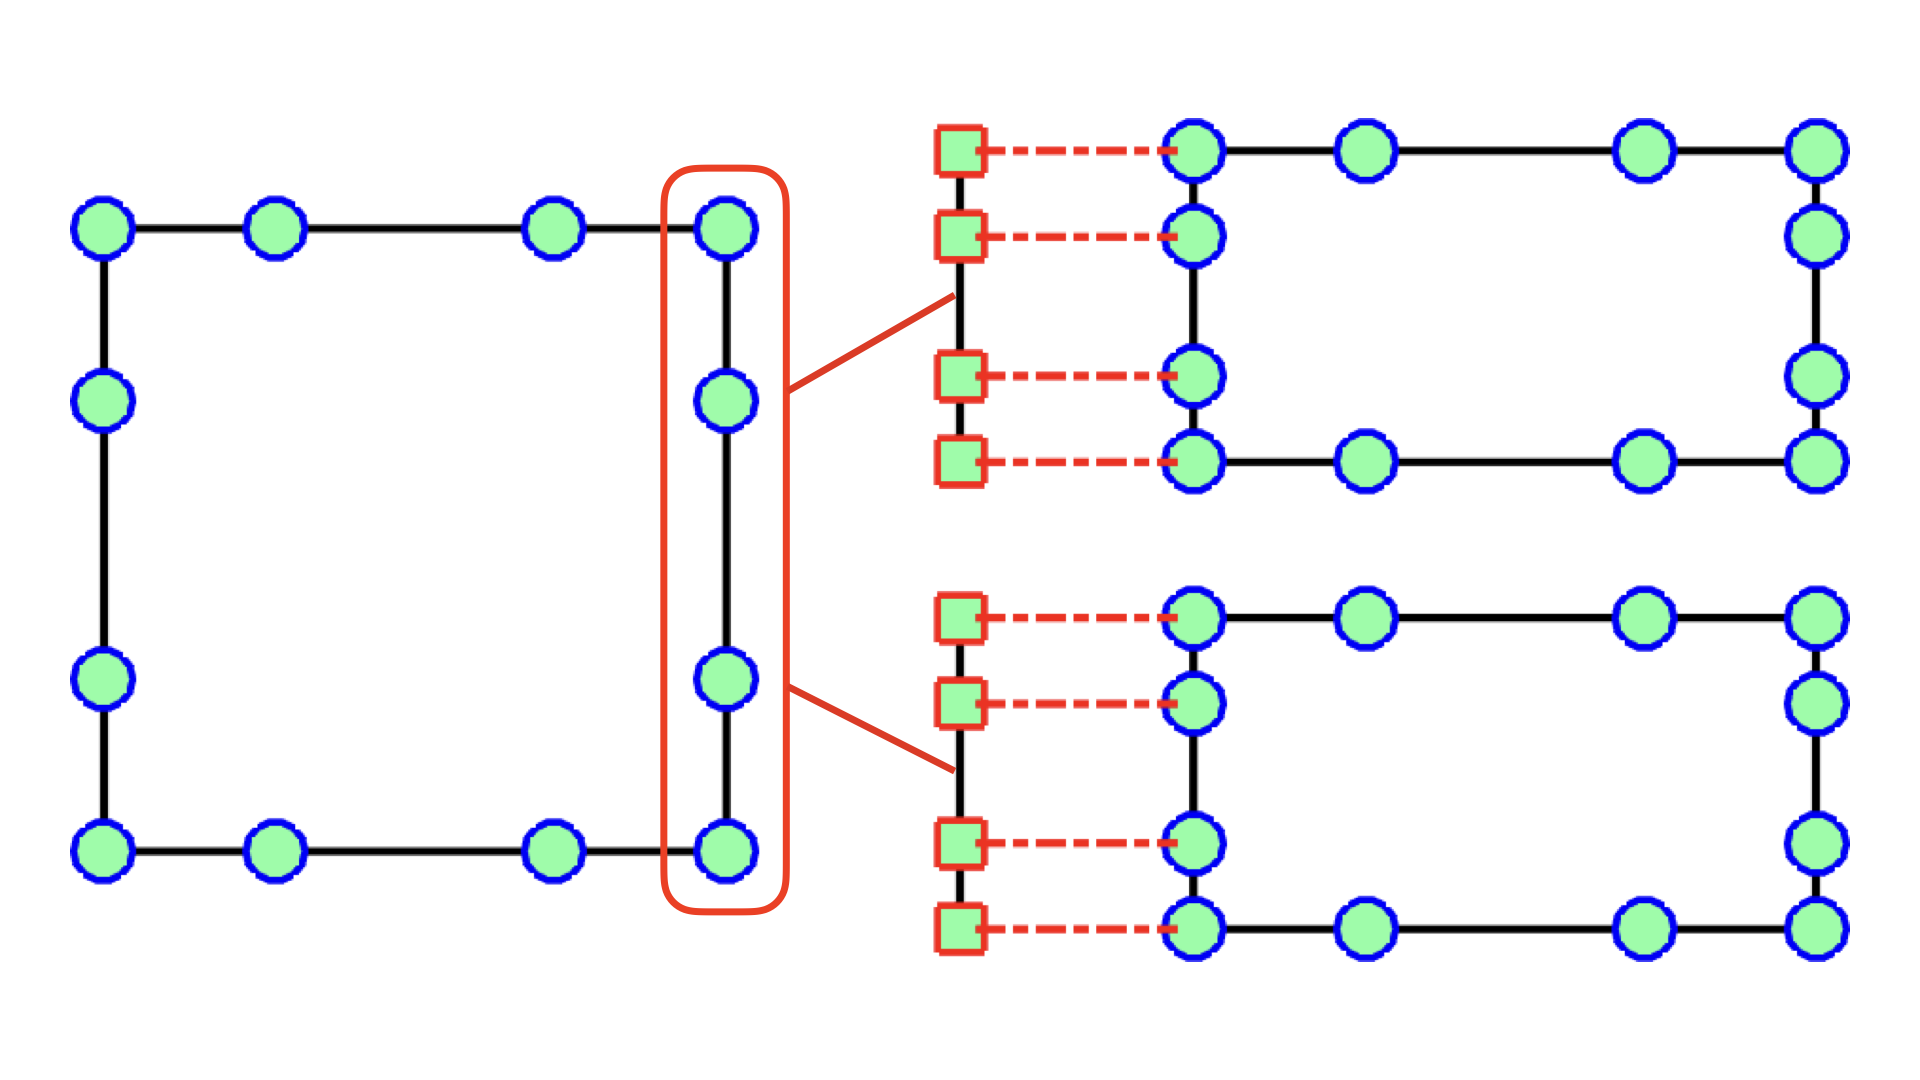
\includegraphics[width=.45\textwidth]{figs/nonconQuad.png}}\label{subfig:noncon1}}
\endgroup
%\subfloat[3D hexahedra-pyramid coupling]{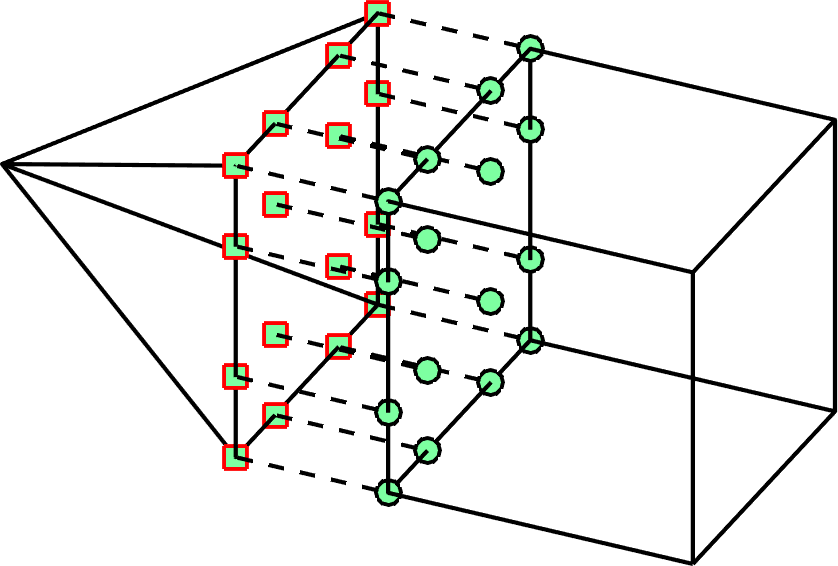
\includegraphics[width=.31\textwidth]{figs/hybrid3D.png}}
\caption{Illustration of two different entropy stable inter-element couplings for $h$ non-conforming meshes.  Each dashed red line indicates a dyadic flux computation required between two nodes. } %The coupling terms in \cite{friedrich2017entropy} requires computing dyadic fluxes between \emph{each} pair of nodes on adjacent interfaces.  The new approach results in a simpler communication pattern between elements. }
\label{fig:noncon}
\end{figure}


\subsection{A variational SBP property}

It can be shown that the SBP property holds for $\bm{D}^i_N$ if the surface quadrature is exact for polynomials of degree $2N$ \cite{chan2017discretely}.  The SBP property is lost if the surface quadrature is only exact for polynomial integrands of degree less than $2N$.  However, one can still show that a variational version of the SBP property is satisfied.  

\begin{lemma}
Let $v\in V^N$, and let the surface trace $\LRl{v}_{\partial \hat{D}} \in V^M\LRp{\partial \hat{D}}$ for some $M \leq N$. If the surface quadrature is exact for polynomials of degree $N+M$,  then for an arbitrary vector $\bm{u}_q$, 
\[
\bm{v}_q^T\bm{Q}_i \bm{u}_q = \bm{v}_q^T\LRp{ \LRp{\bm{V}_f\bm{P}_q}^T \bm{W}_f \diag{{\bm{n}}_i}\bm{V}_f\bm{P}_q - \bm{Q}_i^T}\bm{u}_q
\]
where $\bm{v}$ denotes the vector of values of $v$ of at both volume and surface quadrature points. 
\label{lemma:vsbp}
\end{lemma}
\begin{proof}
Recall that $\bm{Q}_i = \bm{W} \bm{V}_q \bm{D}^i\bm{P}_q$.  Since the volume quadrature is exact for degree $2N-1$ polynomials, we have that
\begin{align*}
\bm{v}_q^T\bm{Q}_i \bm{u}_q &= \bm{v}_q^T\bm{W} \bm{D}^i \bm{P}_q \bm{u}_q = \int_{\hat{D}} \pd{\Pi_N u}{\hat{x}_i} v = \int_{\partial \hat{D}} (\Pi_N u) v \hat{n}_i - \int_{\hat{D}} \LRp{\Pi_N u} \pd{v}{\hat{x}_i}.
\end{align*}
Since the volume integrand $\LRp{\Pi_N u} \pd{v}{\hat{x}_i} \in V^{2N-1}$, it is exactly integrated using the volume quadrature.  Additionally, since $\Pi_N u \in V^N$ and $v\in V^M$ on the surface of $\hat{D}$, the surface quadrature is exact for the surface integral and 
\begin{align*}
&\int_{\partial \hat{D}} (\Pi_N u) v \hat{n}_i -   \int_{\hat{D}} \LRp{\Pi_N u} \pd{v}{\hat{x}_i} =\\
 &\bm{v}_f^T\bm{W}_f{\rm diag}(\hat{\bm{n}}_i) \bm{V}_f\bm{P}_q\bm{u}_q - \LRp{\bm{V}_q\bm{D}^i\bm{P}_q\bm{v}_q}^T\bm{W} \bm{V}_q\bm{P}_q\bm{u}_q\\
=& \bm{v}_q^T \LRp{\bm{V}_f\bm{P}_q}^T\bm{W}_f{\rm diag}(\hat{\bm{n}}_i) \bm{V}_f\bm{P}_q\bm{u}_q - \bm{v}_q^T \bm{P}_q^T\LRp{\bm{D}^i}^T \bm{V}_q^T \bm{W} \bm{V}_q\bm{P}_q\bm{u}_q,
\end{align*}
where we have used that, since $v\in V^N$, $\bm{v}_f = \bm{V}_f\bm{P}_q\bm{v}_q$.  The proof is completed by noting that 
\[
\bm{P}_q^T\LRp{\bm{D}^i}^T \bm{V}_q^T \bm{W} \bm{V}_q\bm{P}_q = \bm{P}_q^T\LRp{\bm{D}^i}^T \bm{M}\bm{P}_q = \bm{P}_q^T\LRp{\bm{D}^i}^T \bm{V}_q^T\bm{W} = \bm{Q}_i^T.
\]
\end{proof}

The variational SBP property also extends to the decoupled SBP operator.  This property, along with the exact differentiation of constants, is necessary for the proof of entropy stability.  
\begin{lemma}
Let $\bm{D}^i_N$ be a decoupled SBP operator on the reference element $\hat{D}$, and let the surface quadrature be exact for polynomials of degree $N+M$ for some $M \leq N$.  Suppose $v\in V^N$ and that $\LRl{v}_{\partial \hat{D}} \in P^M\LRp{\partial \hat{D}}$, Then, 
\[
\bm{v}^T\bm{Q}^i_N\bm{u} = \bm{v}^T\LRp{\bm{B}^i_N - \LRp{\bm{Q}^i_N}^T}\bm{u}.%, \qquad \bm{Q}^i_N \bm{1} = \bm{0}.
\]
where $\bm{v}$ denotes the values of $v$ of at both volume and surface quadrature points.  
\label{lemma:vdsbp}
\end{lemma}
\begin{proof}
For convenience, let $\bm{u}_q, \bm{u}_f$ denote evaluations of $u$ at volume and surface points, such that 
\[
\bm{u} = \begin{pmatrix} \bm{u}_q\\ \bm{u}_f\end{pmatrix}, \qquad \bm{v} = \begin{pmatrix} \bm{v}_q\\ \bm{v}_f\end{pmatrix}.  
\]
The proof of the variational summation by parts property uses the definition of $\bm{Q}^i_N$ (\ref{eq:QN}), 
\begin{align*}
\bm{v}^T\bm{Q}^i_N\bm{u} &= \bm{v}_q^T\bm{Q}_i \bm{u}_q - \frac{1}{2}\LRp{\bm{V}_f\bm{P}_q\bm{v}_q}^T\bm{W}_f\hat{\bm{n}} \LRp{\bm{V}_f\bm{P}_q\bm{u}_q} + \frac{1}{2}\LRp{\bm{V}_f\bm{P}_q\bm{v}_q}^T\bm{W}_f\hat{\bm{n}} \bm{u}_f\\
& - \frac{1}{2}\bm{v}_f^T\bm{W}_f\hat{\bm{n}} \LRp{\bm{V}_f\bm{P}_q\bm{u}_q} + \frac{1}{2}\bm{v}_f^T\bm{W}_f\hat{\bm{n}} \bm{u}_f.
\end{align*}
Applying Lemma~\ref{lemma:vsbp} then yields
\begin{align*}
\bm{v}^T\bm{Q}^i_N\bm{u} =& -\bm{v}_q^T\bm{Q}^T_i \bm{u}_q + \frac{1}{2}\LRp{\bm{V}_f\bm{P}_q\bm{v}_q}^T\bm{W}_f\hat{\bm{n}} \LRp{\bm{V}_f\bm{P}_q\bm{u}_q} + \frac{1}{2}\LRp{\bm{V}_f\bm{P}_q\bm{v}_q}^T\bm{W}_f\hat{\bm{n}} \bm{u}_f\\
&\qquad - \frac{1}{2}\bm{v}_f^T\bm{W}_f\hat{\bm{n}} \LRp{\bm{V}_f\bm{P}_q\bm{u}_q} - \frac{1}{2}\bm{v}_f^T\bm{W}_f\hat{\bm{n}} \bm{u}_f + \bm{v}_f^T\bm{W}_f\hat{\bm{n}} \bm{u}_f\\
=& \begin{pmatrix} \bm{v}_q\\ \bm{v}_f\end{pmatrix}^T 
\left(\begin{pmatrix}
\bm{0}& \\
& \bm{W}_f\diag{\hat{\bm{n}}}
\end{pmatrix}\right.\\
&+
\left.\begin{pmatrix}
-\bm{Q}_i^T + \frac{1}{2}\LRp{\bm{V}_f\bm{P}_q}^T\bm{W}_f\hat{\bm{n}} \bm{V}_f\bm{P}_q & -\frac{1}{2} \LRp{\bm{W}_f\hat{\bm{n}} \bm{V}_f\bm{P}_q}^T\\
\frac{1}{2}\bm{W}_f\hat{\bm{n}} \bm{V}_f\bm{P}_q & -\frac{1}{2}\bm{W}_f\hat{\bm{n}}
\end{pmatrix}  \right)
\begin{pmatrix} \bm{u}_q\\ \bm{u}_f\end{pmatrix}\\
=& \bm{v}^T\LRp{\bm{B}_N - \LRp{\bm{Q}^i_N}^T}\bm{u}.
\end{align*}
\end{proof}
Using Lemma~\ref{lemma:vdsbp}, we will determine the accuracy of the surface quadrature necessary to ensure the proof of semi-discrete entropy stability is valid.  This minimal degree of surface quadrature accuracy will depend on the nature of the reference-to-physical mapping (e.g.\ affine vs curved elements).

\begin{corollary}
\label{lemma:sbpcor}
Let the surface quadrature be exact for polynomials of degree $N$.  Then, 
\[
\bm{1}^T\bm{Q}^i_N\bm{u} = \bm{1}^T\bm{B}_N\bm{u}, \qquad \bm{Q}^i_N\bm{1} = \bm{0},
\]
where $\bm{u}$ is a vector of values of some function at volume and surface quadrature points. %is an arbitrary vector of appropriate size.  
\end{corollary}
\begin{proof}
The proof that $\bm{Q}^i_N \bm{1} = \bm{0}$ follows from the property that polynomials are equal to their $L^2$ projection, and is identical to that of \cite{chan2017discretely,chan2018discretely}.     The proof of the first equality follows from $\bm{Q}^i_N \bm{1} = \bm{0}$ and Lemma~\ref{lemma:vdsbp} with $M=0$
\[
\bm{1}^T\LRp{\bm{Q}^i_N}\bm{u} = \bm{1}^T\LRp{\bm{B}_N - \LRp{\bm{Q}^i_N}^T}\bm{u} = \bm{1}^T{\bm{B}_N}\bm{u}.
\]
\end{proof}
\subsection{Entropy stability on affine meshes}

The high order methods in this work ensure that (\ref{eq:entropyineq}) is satisfied discretely by avoiding the use of the chain rule in the proof of entropy dissipation.  These ``entropy stable'' schemes rely on two main ingredients: an entropy stable numerical flux as defined by Tadmor \cite{tadmor1987numerical} and a concept referred to as ``flux differencing''.  % entropy stable schemes in one-dimension.  
Let $\bm{f}_S\LRp{\bm{u}_L,\bm{u}_R}$ be a numerical flux function which is a function of ``left'' and ``right'' states $\bm{u}_L,\bm{u}_R$.  
The numerical flux $\bm{f}_S$ is \textit{entropy conservative} if it satisfies the following three conditions:  
%The numerical flux $\bm{f}_S$ is an \textit{entropy stable} flux function if it satisfies the following three conditions:  
\begin{gather}
\bm{f}_S(\bm{u},\bm{u}) = \bm{f}(\bm{u}), \qquad \text{(consistency)}\\
\bm{f}_S(\bm{u}_L,\bm{u}_R) = \bm{f}_S(\bm{u}_R,\bm{u}_R), \qquad \text{(symmetry)}\nonumber\\
\LRp{\bm{v}_L-\bm{v}_R}^T\bm{f}_S(\bm{u}_L,\bm{u}_R) = \psi(\bm{u}_L) - \psi(\bm{u}_R), \qquad \text{(conservation)}\nonumber
%\LRp{\bm{v}_L-\bm{v}_R}^T\bm{f}_S(\bm{u}_L,\bm{u}_R) \leq \psi(\bm{u}_L) - \psi(\bm{u}_R), \qquad \text{(entropy dissipation)}\nonumber
\label{eq:esflux}
\end{gather}
%If instead of the third condition, $\bm{f}_S$ satisfies a \emph{stability} property 
%\[
%\LRp{\bm{v}_L-\bm{v}_R}^T\bm{f}_S(\bm{u}_L,\bm{u}_R) \leq \psi(\bm{u}_L) - \psi(\bm{u}_R)$, the flux $\bm{f}_S$ is referred to as \textit{entropy stable}.  

We begin by deriving a skew-symmetric formulation on the reference element $\hat{D}$, and showing it is entropy conservative.  This formulation is then made entropy stable by adding interface dissipation, and can extended in a straightforward manner to affine elements.  The skew-symmetric formulation for (\ref{eq:nonlineqs}) on $\hat{D}$ is 
\begin{gather}
\pd{\bm{u}}{t} + \sum_{i=1}^d \LRs{\begin{array}{cc}
\bm{P}_q & \bm{L}_f\end{array}} \LRp{\LRp{\bm{D}^i_N - \bm{W}_N^{-1}\LRp{\bm{Q}^i_N}^T} \circ \bm{F}_S}\bm{1} + \bm{L}_f \diag{\hat{\bm{n}}}\bm{f}_i^* = 0,\\
\LRp{\bm{F}_S}_{ij} = \bm{f}_S\LRp{\tilde{\bm{u}}_i,\tilde{\bm{u}}_j}, \qquad 1\leq i,j\leq N_q + N^f_q,
\label{eq:esdgSkew}
\end{gather}
where $\bm{f}^*$ is some numerical flux.  Multiplying the formulation (\ref{eq:esdgSkew}) by $\bm{M}$ on both sides yields a weak form 
\begin{gather}
%\bm{M}\pd{\bm{u}}{t} + \sum_{i=1}^d \LRs{\begin{array}{c}
%\bm{V}_q \\ \bm{V}_f\end{array}}^T \begin{pmatrix}
%\bm{W}&\\
%&\bm{W}_f
%\end{pmatrix}
%\LRp{\LRp{\bm{D}^i_N - \bm{W}_N^{-1}\LRp{\bm{Q}^i_N}^T} \circ \bm{F}_S}\bm{1} +  \bm{V}_f^T\bm{W}_f\diag{\hat{\bm{n}}}\bm{f}_i^*\label{eq:esdgSkewWeak}\\
%= 
\bm{M}\pd{\bm{u}}{t} + \sum_{i=1}^d\LRs{\begin{array}{c}
\bm{V}_q \\ \bm{V}_f\end{array}}^T 
\LRp{\LRp{\bm{Q}^i_N - \LRp{\bm{Q}^i_N}^T} \circ \bm{F}_S}\bm{1} + \bm{V}_f^T\bm{W}_f \diag{\hat{\bm{n}}}\bm{f}_i^* = 0.  \label{eq:esdgSkewWeak}
\end{gather}
where the matrix $\LRp{\bm{Q}^i_N - \LRp{\bm{Q}^i_N}^T}$ possesses the following structure
\[
\LRp{\bm{Q}^i_N - \LRp{\bm{Q}^i_N}^T} = \begin{pmatrix}
\bm{Q}_i-\bm{Q}_i^T & \LRp{\bm{V}_f \bm{P}_q}^T\bm{W}_f\diag{\bm{n}_i}\\
\bm{W}_f\diag{\bm{n}_i}{\bm{V}_f \bm{P}_q} & \bm{0}
\end{pmatrix}.
\]

We can now show that the skew-symmetric formulation is semi-discretely entropy conservative.  
\begin{theorem}
Let the surface quadrature be exact for polynomials of degree $N$.  Then, the formulation (\ref{eq:esdgSkew}) is entropy conservative such that
\[
\bm{1}^T\bm{W}\pd{U(\bm{u}_q)}{t} + \sum_{i=1}^d\bm{1}^T\bm{W}_f \diag{\hat{\bm{n}}} \LRp{\psi_i(\tilde{\bm{u}}_f) - \tilde{\bm{v}}_f^T\bm{f}_i^*} = 0, \qquad \bm{u}_q = \bm{V}_q\bm{u}.
\]
\label{thm:esdg}
\end{theorem}
\begin{proof}
Testing (\ref{eq:esdgSkewWeak}) by $\bm{v}_h = \bm{P}_q\bm{v}_q$ yields 
\begin{align}
\bm{v}_q^T\bm{W}\pd{\LRp{\bm{V}_q\bm{u}}}{t} + \sum_{i=1}^d
\tilde{\bm{v}}^T \LRp{\LRp{\bm{Q}^i_N - \LRp{\bm{Q}^i_N}^T} \circ \bm{F}_S}\bm{1} + \tilde{\bm{v}}_f^T \bm{W}_f \diag{\hat{\bm{n}}}\bm{f}_i^* = 0.
\end{align}
One can show that \cite{chan2017discretely}
\begin{align*}
\tilde{\bm{v}}^T \LRp{\LRp{\bm{Q}^i_N - \LRp{\bm{Q}^i_N}^T} \circ \bm{F}_S}\bm{1} &= \tilde{\bm{v}}^T \LRp{\bm{Q}^i_N \circ \bm{F}_S}\bm{1} - \tilde{\bm{v}}^T \LRp{\LRp{\bm{Q}^i_N}^T \circ \bm{F}_S}\bm{1}\\
&= \tilde{\bm{v}}^T \LRp{\bm{Q}^i_N \circ \bm{F}_S}\bm{1} - \bm{1}^T \LRp{{\bm{Q}^i_N} \circ \bm{F}_S}\tilde{\bm{v}}.
\end{align*}
Where we have used that $\bm{F}_S$ is symmetric and that the Hadamard product commutes.  Applying the conservation condition on $\bm{f}_S$ in (\ref{eq:esflux}) then yields
\begin{align*}
\tilde{\bm{v}}^T \LRp{\bm{Q}^i_N \circ \bm{F}_S}\bm{1} - \bm{1}^T \LRp{{\bm{Q}^i_N} \circ \bm{F}_S}\tilde{\bm{v}} &= \sum_{jk} \LRp{\bm{Q}^i_N}_{jk} \LRp{\tilde{\bm{v}}_j-\tilde{\bm{v}}_k} \bm{f}_S\LRp{\tilde{\bm{u}}_j,\tilde{\bm{u}}_k} \\
&= \sum_{ij} \LRp{\bm{Q}^i_N}_{jk} \LRp{\psi_i(\tilde{\bm{u}}_j) - \psi_i(\tilde{\bm{u}}_k)}\\
&= \bm{1}^T\LRp{\bm{Q}^i_N}\psi_i(\tilde{\bm{u}}) - \psi_i(\tilde{\bm{u}})^T\LRp{\bm{Q}^i_N}\bm{1} \\
&= \bm{1}^T\LRp{\bm{Q}^i_N}\psi_i(\tilde{\bm{u}}) = \bm{1}^T\bm{B}^i_N\psi_i(\tilde{\bm{u}}) \\
&= \bm{1}^T\bm{W}_f \diag{\hat{\bm{n}}} \psi_i(\tilde{\bm{u}}_f)
\end{align*}
where we have used Corollary~\ref{lemma:sbpcor} in the second to last equality.
%The final step of the proof is  where we have used Lemma~\ref{lemma:vdsbp} to integrate by parts and conclude that $\bm{1}^T\LRp{\bm{Q}^i_N}^T = 0$.
\end{proof}

\begin{remark}
The only result necessary to prove Theorem~\ref{thm:esdg} is Corollary~\ref{lemma:sbpcor}.  Thus, when generalizing to curved elements, the proof of entropy stability for the skew-symmetric form will depend only on the curved version of Corollary~\ref{lemma:sbpcor}.
\end{remark}

The skew symmetric formulation can also be shown to be locally conservative in the sense of \cite{shi2017local}, which is sufficient to show the numerical solution convergences to the weak solution under mesh refinement.  
\begin{theorem}
The formulation (\ref{eq:esdgSkew}) is locally conservative such that
\begin{align}
\bm{1}^T\bm{W}\pd{\LRp{\bm{V}_q\bm{u}}}{t} + \sum_{i=1}^d\bm{1}^T\bm{W}_f \diag{\hat{\bm{n}}_i}\bm{f}_i^* = 0. 
\end{align}
\end{theorem}
\begin{proof}
To show local conservation, we test (\ref{eq:esdgSkewWeak}) with $1$  %Let $\bm{e}$ be the coefficients of $1$ under the basis $\phi_j(\bm{x})$.
\begin{align}
\bm{1}^T\bm{W}\bm{V}_q\pd{\bm{u}}{t} + \sum_{i=1}^d
\bm{1}^T
\LRp{\LRp{\bm{Q}^i_N - \LRp{\bm{Q}^i_N}^T} \circ \bm{F}_S}\bm{1} + \bm{1}^T\bm{W}_f \diag{\hat{\bm{n}}}\bm{f}_i^* = 0. 
\end{align}
Because $\bm{F}_S$ is symmetric and $\LRp{\bm{Q}^i_N - \LRp{\bm{Q}^i_N}^T}$ is skew-symmetric, the term 
\[
\LRp{\LRp{\bm{Q}^i_N - \LRp{\bm{Q}^i_N}^T} \circ \bm{F}_S}
\]
is a skew-symmetric matrix.  Using that $\bm{A}$, $\bm{x}^T\bm{A}\bm{x} = 0$ for any skew symmetric matrix $\bm{A}$, the volume term vanishes
\[
\bm{1}^T\LRp{\LRp{\bm{Q}^i_N - \LRp{\bm{Q}^i_N}^T} \circ \bm{F}_S}\bm{1} = 0.
\]
% and that the Hadamard product is commutable $\LRp{\bm{A}\circ\bm{B} }^T = \bm{A}^T\circ\bm{B}^T$
%\begin{align}
%\bm{1}^T\LRp{\LRp{\bm{Q}^i_N - \LRp{\bm{Q}^i_N}^T} \circ \bm{F}_S}\bm{1} &= \bm{1}^T\LRp{\bm{Q}^i_N\circ \bm{F}_S}\bm{1} - \bm{1}^T\LRp{\LRp{\bm{Q}^i_N}^T\circ \bm{F}_S}\bm{1}\\
%&= \bm{1}^T\LRp{\bm{Q}^i_N\circ \bm{F}_S}\bm{1} - 
%\bm{1}^T\LRp{\bm{Q}^i_N\circ \bm{F}_S}\bm{1} = 0,
%\end{align}
%where we have used that $\bm{F}_S$ is symmetric.
%\begin{align}
%\end{align}
\end{proof}

Next, we extend this formulation to affinely mapped elements.  Derivatives with respect to physical coordinates on $D^k$ are computed in terms of a change of variables formula and derivatives with respect to reference coordinates 
\[
\pd{u}{x_i} = \sum_{ij} \bm{G}^k_{ij}\pd{u}{\hat{x}_j}, \qquad \bm{G}^k_{ij} = J^k\pd{\hat{x}_j}{{x}_i}, 
\]
where $J^k$ is the determinant of the Jacobian of the geometric mapping on the element $D^k$.
For affine meshes, the scaled geometric terms $\bm{G}^k_{ij}$ are constant over each element.  It was shown in \cite{chan2017discretely} that one can define a physical differentiation matrix as a linear combination of reference differentiation matrices.  Let $\hat{\bm{D}}^i_N$ denote the decoupled SBP operator on the reference element $\hat{D}$, and let the decoupled SBP operators with respect to the physical coordinates on $D^k$ be defined as
\begin{align}
{\bm{D}}^i_N = \sum_{j=1}^d \bm{G}_{ij}\hat{\bm{D}}^j_N.
\end{align}
%Then, $\bm{Q}^i_N = \bm{W} \bm{D}^i_N$ satisfies the SBP property on each element $D^k$
%\begin{equation}
%\bm{Q}^i_N + \LRp{\bm{Q}^i_N}^T = \bm{B}^i_N, \qquad \bm{B}^i_N = \begin{pmatrix}
%\bm{0}&\\
%& {J^k_f}\bm{W}_f \diag{{\bm{n}_i}}
%\end{pmatrix}
%\label{eq:physsbp}
%\end{equation}
%where $J^k_f$ are the Jacobian factors which result from mapping the faces of $D^k$ to reference faces.
%\end{lemma}
Then, an entropy conservative formulation can be given on $D^k$ as follows:
\begin{gather}
\pd{\bm{u}}{t} + \sum_{i=1}^d \LRs{\begin{array}{cc}
\bm{P}_q & \bm{L}_f\end{array}} \LRp{\LRp{\bm{D}^i_N - \bm{W}_N^{-1}\LRp{\bm{Q}^i_N}^T} \circ \bm{F}_S}\bm{1} + \bm{L}_f \diag{{\bm{n}_i}}\bm{f}_i^* = 0, \label{eq:skewform}\\
\LRp{\bm{F}_S}_{ij} = \bm{f}_S\LRp{\tilde{\bm{u}}_i,\tilde{\bm{u}}_j}, \qquad 1\leq i,j\leq N_q + N^f_q, \nonumber\\
\bm{f}^* = \bm{f}_S(\tilde{\bm{u}}_f^+,\tilde{\bm{u}}_f), \qquad \text{ on interior interfaces,} \nonumber
\end{gather}
where $\tilde{\bm{u}}_f^+$ denotes the face value of the entropy-projected conservative variables $\tilde{\bm{u}}_f$ on the neighboring element.  The formulation can be made entropy stable by adding an appropriate penalization term, such as a Lax-Friedrichs or matrix-based dissipation \cite{winters2017uniquely, chen2017entropy, chan2017discretely}.  

\subsection{Curvilinear meshes}

On affine meshes, it is possible to show entropy stability of the skew-symmetric formulation (\ref{eq:esdgSkew}) under a surface quadrature which is only exact for degree $N$ polynomials.  However, on curved meshes, a stronger surface quadrature rule is required to demonstrate entropy stability, where the strength of the surface rule depends on the order and approximation of geometric terms.  

Let $\bm{J}^k\bm{G}^k_{ij}$ denote the vector of scaled geometric terms ${J}^k\bm{G}^k_{ij}$ evaluated at volume and surface quadrature points.  Decoupled SBP operators on a curved element $D^k$  can be defined as in \cite{chan2018discretely} by
\begin{equation}
\bm{D}^i_N = \sum_{j=1}^d \diag{\bm{G}^k_{ij}}\hat{\bm{D}}^j_N + \hat{\bm{D}}^j_N\diag{\bm{G}^k_{ij}}.
\label{eq:dncurved}
\end{equation}
The skew-symmetric formulation (\ref{eq:skewform}) can be extended to curvilinear meshes using the definition of $\bm{D}^i_N$ in (\ref{eq:dncurved}).  However, additional assumptions must be satisfied in order to prove that the resulting formulation is entropy stable.  

\subsection{Discrete geometric conservation law and surface quadrature accuracy}

\note{Add description of how normals factor into this and note that they're computed based on $\bm{G}_{ij}$.}

The first assumption which must be satisfied is the discrete geometric conservation law (GCL) \cite{thomas1979geometric, kopriva2006metric}.  For curved elements, Lemma~\ref{lemma:vdsbp} and Corollary~\ref{lemma:sbpcor} do not necessarily hold at the discrete level.  For example, expanding out the condition $\bm{Q}^i_N\bm{1} = \bm{0}$ in terms of (\ref{eq:dncurved}) yields
\begin{align}
\bm{D}^i_N \bm{1} = \sum_{j=1}^d \diag{\bm{G}^k_{ij}}\hat{\bm{D}}^j_N \bm{1} + \hat{\bm{D}}^j_N\diag{\bm{G}^k_{ij}}\bm{1} = \sum_{j=1}^d \hat{\bm{D}}^j_N\LRp{\bm{G}^k_{ij}} = 0,
\label{eq:dgcl}
\end{align}
where we have used that $\hat{\bm{D}}^j_N \bm{1} = 0$.  For degree $N$ isoparametric mappings, the GCL is automatically satisfied in two dimensions due to the fact that the exact geometric terms $\bm{G}^k_{ij}\in P^{N-1}$ \cite{kopriva2006metric}.  However, in three dimensions, the GCL is not automatically preserved due to the fact that $\bm{G}^k_{ij}\in P^{2N-2}$, and thus cannot be represented exactly using degree $N$ polynomials.  As a consequence, (\ref{eq:dgcl}) must be enforced through an alternative construction of $\bm{G}^k_{ij}$.  

A common approach is to rewrite the geometric terms as the curl of some quantity $\bm{r}^i$, but to interpolate $\bm{r}^i$ before applying the curl \cite{visbal2002use, kopriva2006metric, hindenlang2012explicit}:
\begin{align}
\bm{r}^i = { \pd{\bm{x}}{\hat{x}_i}\times \bm{x}}, \qquad
\LRs{\begin{array}{c}
\bm{G}^k_{i1}\\
\bm{G}^k_{i2}\\
\bm{G}^k_{i3}\end{array}} = -\frac{1}{2}\LRp{\pd{I_{R}\bm{r}^k}{\hat{x}_j}-\pd{I_{R}\bm{r}^j}{\hat{x}_k}}, 
\label{eq:iconscurl}
\end{align}
where $I_{R}$ denotes a degree ${R}$ polynomial interpolation operator with appropriate interpolation nodes.\footnote{This interpolation step must be performed using interpolation points with an appropriate number of nodes on each boundary \cite{chan2018discretely}.  These include, for example, GLL nodes on tensor product elements, as well as Warp and Blend nodes on non-tensor product elements \cite{warburton2006explicit, chan2015comparison}.}  Because the geometric terms are computed by applying the curl, both $\bm{G}^k_{ij}$ and $n_iJ^f$ are approximated using degree $(R-1)$ polynomials.  

Because $\bm{D}^i_N$ are now defined through (\ref{eq:dncurved}), Corollary~\ref{lemma:sbpcor} and the proof of entropy stability may not hold for curved elements and must be modified.  The introduction of curvilinear meshes will impose slightly different conditions on the accuracy of the surface quadrature, which are summarized in the following curved version of Corollary~\ref{lemma:sbpcor}.
\begin{lemma}
Assume that the geometric terms $\bm{G}_{ij} \in V^N$ satisfy the discrete GCL (\ref{eq:dgcl}), that $\LRl{\bm{G}_{ij}}_{\partial \hat{D}}\hat{n}_j \in V^R\LRp{\partial \hat{D}}$, and that the surface quadrature is exact for polynomials of degree $N+R$.  Then, 
\[
\bm{1}^T\bm{Q}^i_N\bm{u} = \bm{1}^T\bm{B}^i_N \bm{u}, %\qquad \bm{B}^i_N = \begin{pmatrix}
%\bm{0}& \\
%& \bm{W}_f\diag{\bm{n}_i}
%\end{pmatrix}, 
\qquad \bm{Q}^i_N \bm{1} = 0, 
\]
where 
\[
\bm{B}^i_N =  \begin{pmatrix}
\bm{0}&\\
& {J^k_f}\bm{W}_f \diag{{\bm{n}_i}}
\end{pmatrix}.
\]
\label{lemma:vdsbpcurved}
\end{lemma}
\begin{proof}
The second equality $\bm{Q}^i_N \bm{1} = 0$ is a consequence of the discrete GCL (\ref{eq:dgcl}), and the proof is identical to that of \cite{chan2018discretely}.  For the first equality, if the surface quadrature is exact for polynomials of degree $2N$ on the trace space, then the stronger matrix SBP property $\bm{Q}^i_N = \bm{B}^i_N - \LRp{\bm{Q}^i_N}^T$ holds \cite{chan2018discretely}.  Combining this with $\bm{Q}^i_N\bm{1} = 0$ yields the desired result.  We focus on the proof of the variational SBP property for surface quadrature which are exact for polynomials of degree $N+R < 2N$.  

Expanding $\bm{1}^T\bm{Q}^i_N\bm{u}$ yields
\[
\bm{1}^T\bm{Q}^i_N\bm{u} = \frac{1}{2}\sum_{j=1}^d \bm{1}^T \diag{\bm{G}_{ij}} \hat{\bm{Q}}^j_N \bm{u} + \bm{1}^T\hat{\bm{Q}}^j_N \diag{\bm{G}_{ij}} \bm{u}. %=  \frac{1}{2}\sum_{j=1}^d \bm{1}^T \diag{\bm{G}_{ij}} \hat{\bm{Q}}^j_N \bm{u},
\]
For the latter term in the sum, Lemma~\ref{lemma:vdsbp} holds and
\begin{align}
\sum_{j=1}^d\bm{1}^T\hat{\bm{Q}}^j_N \diag{\bm{G}_{ij}} \bm{u} &= 
\sum_{j=1}^d\bm{1}^T\LRp{\hat{\bm{B}}^j_N - \LRp{\hat{\bm{Q}}^j_N}^T} \diag{\bm{G}_{ij}} \bm{u} \\
&= \sum_{j=1}^d\bm{1}^T\hat{\bm{B}}^j_N\diag{\bm{G}_{ij}}\bm{u}, \nonumber
\label{eq:vsbp1}
\end{align}
where we have used that $\hat{\bm{Q}}^j_N \bm{1} = \bm{0}$.  For the former term in the sum, we expand out 
\begin{gather}
\sum_{j=1}^d\bm{1}^T \diag{\bm{G}_{ij}} \hat{\bm{Q}}^j_N \bm{u} = 
\sum_{j=1}^d{\bm{G}_{ij}}^T \hat{\bm{Q}}^j_N \bm{u} \\
= \sum_{j=1}^d\begin{bmatrix}
\bm{G}^q_{ij}\\
\bm{G}^f_{ij}
\end{bmatrix}^T \begin{bmatrix} 
\hat{\bm{Q}}_i - \frac{1}{2}\LRp{\bm{V}_f \bm{P}_q}^T  \bm{W}_f{\rm diag}(\hat{\bm{n}}_i) \bm{V}_f\bm{P}_q &  \frac{1}{2}\LRp{\bm{W}_f{\rm diag}(\hat{\bm{n}}_i)\bm{V}_f\bm{P}_q}^T\label{eq:ibpg}\\
-\frac{1}{2}\bm{W}_f{\rm diag}(\hat{\bm{n}}_i)\bm{V}_f\bm{P}_q & \frac{1}{2}\bm{W}_f{\rm diag}(\hat{\bm{n}}_i)
\end{bmatrix} \begin{bmatrix}\bm{u}_q\\
\bm{u}_f\end{bmatrix}.\nonumber
\end{gather}
where $\bm{G}^q_{ij},\bm{G}^f_{ij}$ denote the values of $\bm{G}_{ij}$ at volume and surface quadrature points.  

Because $\bm{G}_{ij} \in V^N$, it is equal to its own $L^2$ projection, and the values at volume and surface quadrature points are related by $\bm{G}^f_{ij} = \bm{V}_f\bm{P}_q\bm{G}^q_{ij}$.  We can use this to simplify (\ref{eq:ibpg})
\begin{align*}
\bm{1}^T \diag{\bm{G}_{ij}} \hat{\bm{Q}}^j_N \bm{u} =&  \LRp{\bm{G}^q_{ij}}^T { \bm{Q}_i}  \bm{u}_q - \frac{1}{2} \LRp{{\bm{V}_f \bm{P}_q}\bm{G}_{ij}^q+\bm{G}^f_{ij}}^T{\bm{W}_f{\rm diag}({\bm{n}}_i)\bm{V}_f\bm{P}_q}\bm{u}_q\\
&+ \frac{1}{2} \LRp{{\bm{V}_f \bm{P}_q}\bm{G}_{ij}^q+\bm{G}^f_{ij}}^T\frac{1}{2}\bm{W}_f{\rm diag}({\bm{n}}_i)\bm{u}_f\\
=& \LRp{\bm{G}^q_{ij}}^T \LRp{ \hat{\bm{Q}}_i - \LRp{{\bm{V}_f \bm{P}_q}\bm{G}_{ij}^q}^T{\bm{W}_f{\rm diag}(\hat{\bm{n}}_i)\bm{V}_f\bm{P}_q}}\bm{u}_q \\
&+ \LRp{\bm{G}^f_{ij}}^T\bm{W}_f{\rm diag}(\hat{\bm{n}}_i)\bm{u}_f. %\\
%&= \LRp{\bm{G}^q_{ij}}^T \LRp{ \LRp{{\bm{V}_f \bm{P}_q}\bm{G}_{ij}^q}^T{\bm{W}_f{\rm diag}({\bm{n}}_i)\bm{V}_f\bm{P}_q}}\bm{u}_q + \LRp{\bm{G}^f_{ij}}^T\bm{W}_f{\rm diag}({\bm{n}}_i)\bm{u}_f 
\end{align*}
The first term can be further simplified using Lemma~\ref{lemma:vsbp}
\[
\LRp{\bm{G}^q_{ij}}^T \LRp{ \hat{\bm{Q}}_i - \LRp{{\bm{V}_f \bm{P}_q}\bm{G}_{ij}^q}^T{\bm{W}_f{\rm diag}(\hat{\bm{n}}_i)\bm{V}_f\bm{P}_q}}\bm{u}_q = \LRp{\bm{G}^q_{ij}}^T \LRp{ \hat{\bm{Q}}_i}^T\bm{u}_q.
\]
The latter term can be combined with the surface term of (\ref{eq:vsbp1}) by noting that 
\[
\LRp{\bm{G}^f_{ij}}^T\bm{W}_f \diag{\hat{\bm{n}}_i}\bm{u}_f =\bm{1}^T\hat{\bm{B}}^j_N\diag{\bm{G}_{ij}}\bm{u} = \bm{1}^T\diag{\bm{G}_{ij}}\hat{\bm{B}}^j_N\bm{u},
\]
where we have used that $\hat{\bm{B}}^j_N$ is diagonal and commutes with diagonal scaling by $\bm{G}_{ij}$.
%as $\LRp{\bm{G}^f_{ij}}^T\bm{W}_f{\rm diag}({\bm{n}}_i)\bm{u}_f = \bm{1}^T\hat{\bm{B}}^j_N \bm{u}$.  
We can use polynomial exactness and the fact that the geometric terms satisfy the continuous GCL by construction \cite{chan2018discretely} to show that $\sum_{j=1}^d  \hat{\bm{Q}}_j {\bm{G}^q_{ij}} = 0$.
Combining this with (\ref{eq:vsbp1}) and expanding out $\hat{\bm{B}}^j_N$ yields that
\begin{align*}
\bm{1}^T\bm{Q}^i_N\bm{u} &= \sum_{j=1}^d \LRp{
\frac{1}{2}\LRp{\bm{G}^q_{ij}}^T \LRp{ \hat{\bm{Q}_i}}^T \bm{u}_q + \bm{1}^T\begin{pmatrix}
\bm{0} &\\
& \bm{W}_f \diag{\bm{G}_{ij} \circ \hat{\bm{n}}_j}
\end{pmatrix}
\bm{u}} \\
&=  \bm{1}^T\begin{pmatrix}
\bm{0} &\\
& \bm{W}_f \diag{\sum_{j=1}^d \bm{G}_{ij} \circ \hat{\bm{n}}_j}
\end{pmatrix}
\bm{u} = \bm{1}^T\bm{B}^i_N\bm{u}.
\end{align*}
where we have used in the final step that $\sum_{j=1}^d\bm{G}_{ij}\hat{n}_j = \bm{n}_i J^k_f$ \cite{ciarlet1978finite, chan2018discretely}
\end{proof}

Lemma~\ref{lemma:vdsbpcurved} implies that the polynomial degree $R$ of the surface geometric terms must be compatible with the accuracy of the surface quadrature.  This, in turn, will depend on the way in which geometric terms are approximated.  \note{Finish.}

%\end{proof}
%Thus, if geometric terms are approximated using degree $N$ polynomials as in \cite{kopriva2006metric}, then the skew-symmetric formulation with composite GLL quadrature can be used. 


%\subsection{Simplicial vs tensor product elements}
%
%It was shown in \cite{chan2018discretely} that the approximation error is $O\LRp{h^{R+1}}$, and that taking $R = (N+1)$ approximates the geometric terms with an error of $O(h^{N+2})$.
%
%\note{Need to note image of curl is in different spaces for simplicial vs tensor product elements.  Influences proofs that geometric terms satisfy appropriate assumptions in those cases.}
%%\subsection{On implementation and computational cost}
%
\note{Kopriva trick to enforcing GCL still results in $Q^N$ normals 3D.  May not satisfy requirement that $\bm{1}^T\bm{Q}^i_N \psi_i(\tilde{\bm{u}}) = \bm{1}^T\bm{B}^i_N \psi_i(\tilde{\bm{u}})$ because of quadrature inaccuracy.  Note - this still works regardless for conforming hexes because of the full matrix SBP property.}  

\section{Numerical experiments}

In this section, we present two-dimensional experiments on hybrid meshes consisting of quadrilaterals and triangles, as well as on non-conforming meshes of quadrilateral elements.  

\subsection{Reduced surface quadrature}

\note{Affine and curved triangles with GLL surface quadrature (under-integrated).}

\subsection{Hybrid meshes}

\subsection{Non-conforming meshes}


%\appendix
%
%\section{An explicit skew-symmetric entropy stable formulation for DG-SEM} 
%
%\note{$\bm{V}_q,\bm{P}_q = \bm{I}$, while $\bm{V}_f$ reduces to a permutation matrix.  }
%
%\note{For non-conforming faces, need to interpolate entropy variables to form fluxes.  Given this info, can rotate from skew form to strong form using mortar variables.  }

\bibliographystyle{unsrt}
\bibliography{dg}


\end{document}


